\documentclass{standalone}
\usepackage{tikz}
\usepackage{ctex,siunitx,bm}
\setCJKmainfont{Noto Serif CJK SC}
\usepackage{tkz-euclide,ninecolors}
\usepackage{amsmath}
\usetikzlibrary{patterns, calc}
\usetikzlibrary {decorations.pathmorphing, decorations.pathreplacing, decorations.shapes,}
\begin{document}
\small
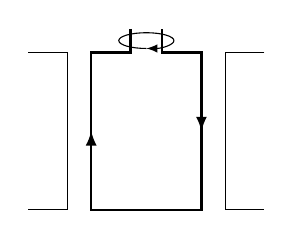
\begin{tikzpicture}[>=latex,yscale=1.0]
  \draw(-1.5,1.5)--++(0.5,0)--++(0,-2)--++(-0.5,0);
  \draw(1.5,1.5)--++(-0.5,0)--++(0,-2)--++(0.5,0);
  \draw[thick](-0.2,1.8)--++(0,-0.3)--++(-0.5,0)--++(0,-2)--++(1.4,0)--++(0,2)--++(-0.5,0)--++(0,0.3);
  % \node at (-1.2,0.5){$N$};
  % \node at (1.2,0.5){$S$};
  \draw[thick,->] (0.7,1.5)--(0.7,0.5);
  \draw[thick,->] (-0.7,-0.5)--(-0.7,0.5);
  \draw[thin,-latex](0,1.55)arc [start angle=270,end angle=-90,x radius=.35,y radius=.1];
\end{tikzpicture}
\end{document}